\taskpic{ В цилиндрическом стакане находилось 4
  шарика. Экспериментатор аккуратно с помощью шприца добавлял в стакан
  жидкость и заносил в таблицу значения высоты уровня жидкости в
  стакане в зависимости от объёма добавленной жидкости. Известно, что
  в процессе эксперимента шарики не всплывали. По результатам
  измерений определите площадь сечения стакана и объём одного
  шарика. }
{
  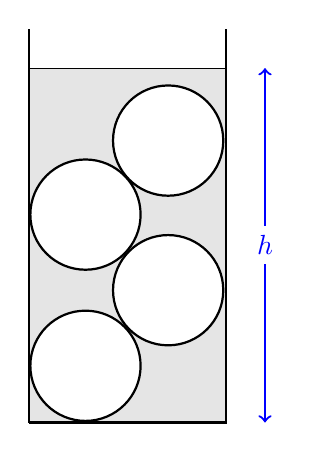
\begin{tikzpicture}
    \draw[fill=gray!20] (0,0) rectangle ++(2.5,4.5);
    \draw[thick] (0,0) -- ++(2.5,0) -- ++(0,5);
    \draw[thick] (0,0) -- ++(0,5);
    \draw[fill=white,thick] (0.72,0.72) circle (0.7cm);
    \draw[fill=white,thick] (1.77,1.68) circle (0.7cm);
    \draw[fill=white,thick] (0.72,2.64) circle (0.7cm);
    \draw[fill=white,thick] (1.77,3.58) circle (0.7cm);
    \draw[thick,blue,<->] (3,0) -- (3,4.5) node[midway,fill=white] {$h$}; 
  \end{tikzpicture}
}

\begin{table}[h]
  \centering
  \large
  \begin{tabular}{|c|c|c|c|c|c|c|c|c|c|c|c|c|c|}
    \hline
    $V,\unit{см}^3 $ & 0 & 50 & 100 & 150 & 200 & 250 & 300 & 350 & 400
    & 450 & 500 & 550 & 600\\
    \hline
    $h, \unit{см}$ & 0 & 1,2 & 2,7 & 4,1 & 5,3 & 7,0 & 9,0 & 10,5 &
                                                                     12,0
    & 13,0 & 14,0 & 15,0 & 16,0  \\
    \hline
  \end{tabular}
\end{table}
% Максвелл-2016, 8 класс
% ccpe-2016-2017-8